\chapter{Conclusions and Future Work }
\label{chap:Intro}
\textit{In this chapter raise the principal conclusion of this work and present the future experiments on these structures in the wake of obtained results.}
\vfill
\minitoc
\newpage
\allowdisplaybreaks


\lettrine[lines=3, lraise=.1, nindent=0mm, slope=0mm]{\textbf{T}}{he} aim of this work finally resulted in important publications, the CQWs continue to be an excellent platform to study optical and quantum-mechanical properties.
This work presents an important result and enhances the importance of studying these structures. The principal idea to expose our results was planned to simplify but specify the physical basis, starting by explaining a single QW and structural properties and then raising the relevance of symmetry context to understand the physical behavior of electrons.
We also exposed the symmetry importance of this work and its fundamental role in
the emergence of the \gls{oa}. Then focus on symmetry reduction (symmetry breaking) which is the cause of the appearance of interesting physical properties, in our case optical properties.
The perturbative model proposed to understand the IOA is simple yet very
useful, as this mainly depends on the grade of asymmetry in the CQWs system, the
more asymmetry, the bigger the RAS signal. Also, this model is supported by numerical
calculations with a good approximation
% The perturbative model purposed to understand the \gls{oa} is simple yet very useful, as this mainly depends on the grade of asymmetry in the CQWs system, the more asymmetry increases the RAS signal. Also, this model is supported by numerical calculations with a good approximation. 
When we had obtained the results of the first, we purposed to develop codes to generate numerical results and although this represented a new area to explore, we decided to dedicate enough time to get a new tool to support our experimental work.\\
Already inside in numerical solutions area, we realized the complexity of generating reliable
results, and the overall existence of numerous proposals to get it, then we decided to implement the simple context. Our numerical results are simple but reliable in accordance with the experimental energies and, by this reason we create a  \href{https://github.com/lflmgroup}{GitHub} repository \cite{lflmgroup} with the aim to develop new codes and numerical models that in future work can be implemented.



In the experimental part, the results are proof of the arduously work that it was inverted, along with the project it was realized experiments to study and understand the physics which involves the CQWs systems, although this has been studied for several years ago, our contribution it is novel.

The quantum confinement is the key to these structures, if we consider the symmetry breaking by coupled wells width asymmetry exhibits wonderful physics, from spin dynamics to excitonic effects. With respect to spin dynamics into CQWs structures, it was realized
experiments of circularly polarized PL over the samples shown in this work, reveal that the
spin relaxation time $\tau_s$. It has been demonstrated that the degree of circular polarization is directly related to the asymmetry of the CQWs \cite{bravo2022photoluminiscence}.

The excitonic properties shown in the \Cref{subsubsec:chapter-3-PR-exciton-effects} are really interesting, the PR
experiments performed as a laser power function reveal a non-common transition in these experiments, this transition associated with a trion, commonly occurs in structures under external disturbance as an electric field is applied, in our case, we not only detect the trion transition, but also it modulated with a light source. This means this can be applied as a laser transistor. These \gls{PR} results are very relevant, in fact as future work we planned
to publish them.

Finally, in the RAS experiments it is clearly the wonderful physics that exhibits ACQWs
structures, the results obtained are the principle of an experiments series which we are
thinking to carry out. Without the intention of being repetitive since the results prove our work, we purpose to take further the RAS technique to explore with more detail the ACQWs structures. The first upgrade of RAS experiments, it is do it spin sensitive, which means, spin-resolved RAS experiments.
The principal idea is to enhance the RAS setup to measure spin response. Our proposal is to carry out the experiments just by changing the modulated PEM polarization. In the RAS setup (as can see in \Cref{fig:chapter-3-ras-setup}) the monochromatic beam is first polarized to then modulated linear polarization by the PEM between mutual perpendicular polarization states, to finally spot on sample along  $[110]$ and $[1\overline{1}0]$  directions. Then, in the spin resolve RAS experiments, it is purposed to modify PEM polarization modulation, to this it is possible
to the choice that the modulation being right circular and left circular polarization, in the
PEM device this is $\lambda/4$ and $3\lambda/2$ which in contrast with the $\lambda/2$ of the traditional RAS
experiments.
\begin{figure}[H]
	\floatbox[{\capbeside\thisfloatsetup{capbesideposition={right,top},capbesidewidth=0.4\textwidth}}]{figure}[0.95\FBwidth]
	{ \caption{ Spin resolve RAS experiments worked on ACQWs-2 sample, this experiments carried out in sequential way, firstly measured with one polarization state and then the second state. The sample it was placed along preferential direction ($[1\overline{1}0]$), maybe this be a reason can observer a structural signal of RAS, this means, the line shape of  anisotropy due to the asymmetry structure. Although, it's notable the difference between mutual polarization states.
	}\label{fig:chapter-4-subsec-conclusion-ras-spin-1}}
	{
	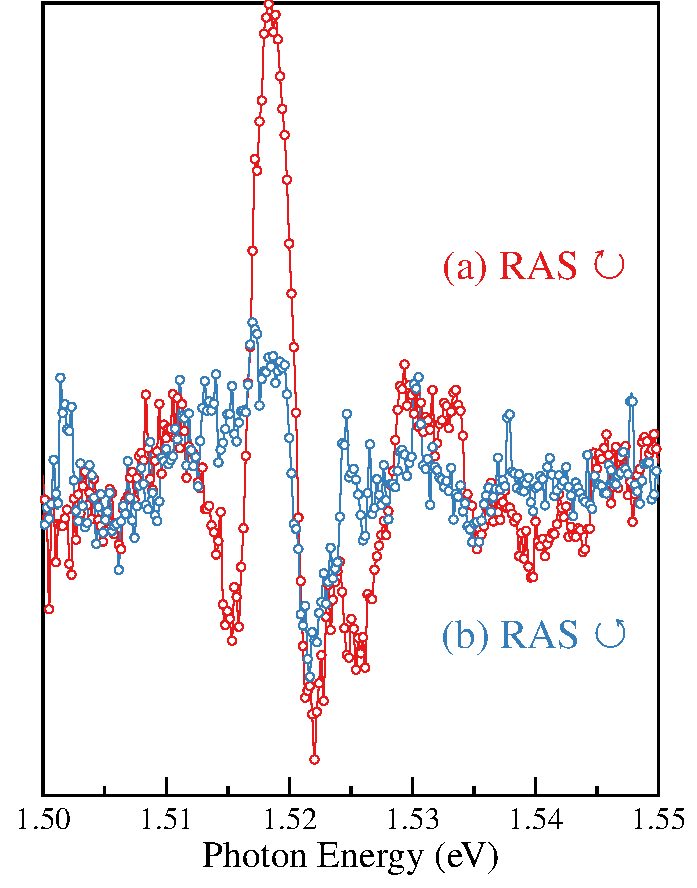
\includegraphics[width=0.6\textwidth]{../figures/chapter-4/ras-spin/out/ras-spin-1.pdf}
	}
\end{figure}
The first results obtained from worked on ACQWs-2 sample shows in \Cref{fig:chapter-4-subsec-conclusion-ras-spin-1}, these experiments were it performed with the sample position in a preferential direction $[110]$
and as a sequential way, this means, firstly with a polarization state then the other state.
The results shown in \Cref{fig:chapter-4-subsec-conclusion-ras-spin-1} are the average of sequential experiments, each of one with
their respective polarization. The signals results exhibit an interest difference, although,
maybe the line-shape has a remainder of structural anisotropy due to the asymmetry in
the structure ($C_{2v}$). If taken into account the contribution of structural anisotropy, it appears to be polarization is longer. Even if, these results are really first approximation, the technique has powerful to explore spin properties. The second RAS upgrade to spin resolve, it is a proposal, instead of polarization states with the PEM will be used a laser beam circular (left and right) focused onto the sample, while the RAS signal it’s measured traditionally. We expected that these upgrades the RAS experiments, turning a tool for spin study.



% \lettrine[lines=3, lraise=.1, nindent=0mm, slope=0mm]{\textbf{T}}{he} aim of this work finally results in important publications, the \gls{CQWs} continue to be an excellent platform to study optical and quantum-mechanical properties, this work presents an important result and enhance the importance of study these structures. The principal idea to exposes our results was planned to simplify but specify the physical basis, starting from explain a single QW and structural properties then raise the relevance of symmetry context to understand the physical behavior of electrons. In section exposes the symmetry importance in this work and their fundamental role in emergence of the \gls{oa}. Then focus on symmetry reduction (symmetry breaking)  which is the causes of appearance  of interesting physical properties, in our case optical properties. 

% The perturbative model purposed to understand of the \gls{oa} is simple and useful, as this depend on grade of asymmetry in the CQWs system, the more asymmetry increases the RAS signal. Also, this model is support by the numerical calculations with a good approximation. When it had obtained the firsts results, we purposed to developed  codes to generate numerical results and although this represented a new area to explore, we decided to dedicated enough time to get a new tool to support our experimental work. Already inside in numerical solutions' area, we realized of complexity of  generate reliable results, overall to existence of numerous proposals to get it, then we decided implemented the simplicity context. Our numerical results are simple but  reliable in accordance with the numerical results, by this reason we create a \href{https://github.com/lflmgroup}{GitHub} repository\cite{lflmgroup} with aim to developed new codes and numerical models which in future work can will be implemented. In the experimental part, the results are the proof of the arduously work that it was inverted, along of the project it was realized experiments to study and understand the physics which involves the \gls{CQWs} systems, although this has been study for several years ago, our contribution it's novel. \\*
% The quantum confinement is the key of these structures, if add the symmetry breaking by coupled wells width asymmetry exhibits wonderful physics, from spin dynamics to excitonic effects. With respect to spin dynamics into CQWs structures, it was realized experiments of circularly polarized PL over the samples shown in this work, reveals that the spin relaxation time $\tau_{s}$. It has been demonstrates that the degree of circular polarization is directly related to the asymmetry of the \gls{CQWs}\cite{bravo2022photoluminiscence}. \\*
% The excitonic properties shown in the \Cref{subsubsec:chapter-3-PR-exciton-effects} are really interesting, the \gls{PR} experiments performed as a laser power function reveal a non-common transition in these experiments, this transition associated with a trion, commonly occurs in structures under external disturbance as an electric field applied, in our case, we not only detect the trion transition, but also it modulated with a light source.  This means this can be applied as a laser transistor. These  PR results are very relevant, in fact as a future work we planned to publish them. 

% Finally, in the RAS experiments  it's clearly the wonderful physics which exhibits ACQWs structures, the results obtained are the principle of an experiments' series  which we're thinking to carried out. Without intention to being  repetitive since the results proofs our hard work, we purpose to take further the RAS technique to explore with more detail the ACQWs structures. The first upgrade of RAS experiments, it's do it spin sensitive, this means, spin resolve RAS experiments. \\
% The principal idea is enhancing the RAS setup to measure spin response. Our proposal is to carry out the experiments just changing the modulated PEM polarization. In the RAS setup (as can see in \Cref{fig:chapter-3-ras-setup}) the monochromatic beam is first polarized to then  modulated linear polarization by the PEM between mutual perpendicular polarization states, to finally spot on sample along $[110]$ and $[1\overline{1}0]$ directions. Then, in the spin resolve RAS experiments, it purpose to modify PEM polarization modulation, to this it's possible to choice that the modulation being right circular and left circular polarization,  in the PEM device this is $\lambda/4$ and $3\lambda/2$ which in contrast with the  $\lambda/2$ of the traditional RAS experiments.  

% The first results obtained from worked on ACQWs-2 sample shows in \Cref{fig:chapter-4-subsec-conclusion-ras-spin-1}, these experiments were it performed with the sample position in a preferential direction $[1\overline{1}0]$ and as a sequential way, this means, firstly with a polarization state then the other state. The results shown in \Cref{fig:chapter-4-subsec-conclusion-ras-spin-1} are the average of sequential experiments, each of one with their respective polarization. The signals results exhibit an interest difference, although, maybe the  line-shape has a remainder of structural anisotropy due to the asymmetry in the structure ($C_{2v}$).  If taken into account the contribution of structural anisotropy, it appears to be polarization is  longer. Even if, these results are really first approximation, the technique has powerful to explore spin properties. 
% The second \gls{RAS} upgrade to  spin resolve, it's a proposal, instead of polarization states  with the \gls{pem} will be used a laser beam circular (left and right)  focused onto the sample, while the \gls{RAS} signal it's measured traditionally. 
% We expected that these upgrades the RAS experiments, turning a  tool for spin study. 









